\documentclass{standalone}
\usepackage{pgfplots}
\pgfplotsset{compat=newest}
\usepgfplotslibrary{ternary}
\begin{document}
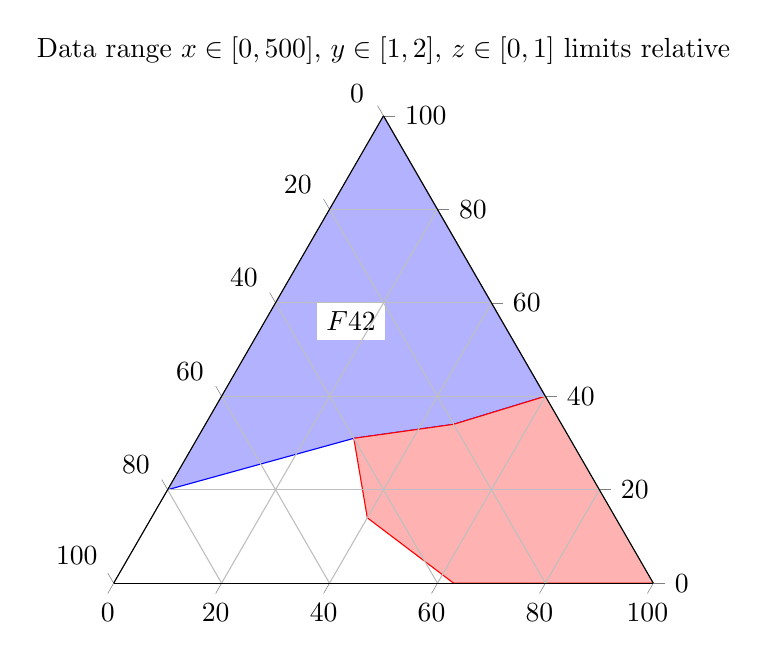
\begin{tikzpicture}
\begin{ternaryaxis}[
	xmax=500,ymin=1,ymax=2,
	ternary limits relative,
	title={Data range $x\in[0,500]$, 
		$y\in[1,2]$, $z\in[0,1]$ limits relative},
	area style]
\addplot3 coordinates {
	(100,1.8,0)
	(155,1.4,0.29)
	(170,1.2,0.46)
	(200,1,0.6)
	(500,1,0)
};
\addplot3 coordinates {
	(200,1,0.6)
	(170,1.2,0.46)
	(155,1.4,0.29)
	(70,1.46,0.4)
	(0,1.37,0.63)
	(0,1,1)
};
\node[fill=white] 
	at (axis cs:280,1.28,0.16) {$F 42$};
\node[fill=white] 
	at (0.7,0.2) {$F 43$};
\end{ternaryaxis}
\end{tikzpicture}
\end{document}
